\chapter{System design and implementation}\label{chap:system}
This chapter presents the concrete design and implementation of the SmartEdu system, translating the methodology outlined in Chapter~\ref{chap:methodology} into a 
functioning software implementation. Such implementation are generalized in Figure~\ref{fig:pipeline}, an illustration of three principal flow paths through the system, functioning as a complete summarization of the 
operational pipeline.

\begin{figure}[H]
\centering
\resizebox{\textwidth}{!}{%
\begin{tikzpicture}[
  node distance=0.8cm and 1.0cm,
  box/.style={draw, rounded corners=3pt, minimum height=0.6cm, align=center, font=\tiny, fill=#1},
  db/.style={cylinder, draw, shape border rotate=90, minimum width=1.2cm, minimum height=0.7cm, font=\tiny, fill=#1, aspect=0.25},
  arr/.style={->, >=stealth, thick},
  lbl/.style={font=\tiny, midway, above},
  phase/.style={font=\footnotesize\bfseries, text=#1},
]
% === Path 1: Knowledge Ingestion ===
\node[phase=blue!70] at (0, 5.5) {Knowledge Ingestion};
\node[box=gray!15] (pdf) at (0, 4.8) {Raw PDF};
\node[box=blue!12] (parser) at (2.5, 4.8) {Parser};
\node[box=blue!12] (llm) at (5.0, 4.8) {LLM Extraction};
\node[box=blue!12] (builder) at (7.5, 4.8) {Graph Builder};
\node[db=purple!12] (neo_k) at (10.5, 5.3) {Neo4j};
\node[db=red!12] (milvus) at (10.5, 4.3) {Milvus};
\node[db=yellow!15] (minio) at (2.5, 3.8) {MinIO};
\draw[arr] (pdf) -- (parser);
\draw[arr] (parser) -- (llm);
\draw[arr] (llm) -- (builder);
\draw[arr] (builder) -- node[lbl]{entities} (neo_k);
\draw[arr] (builder) -- node[lbl, below]{embeddings} (milvus);
\draw[arr] (pdf) -- node[lbl, left]{archive} (minio);
% === Path 2: Student Lifecycle ===
\node[phase=green!60!black] at (0, 2.5) {Student Lifecycle};
\node[box=gray!15] (login) at (0, 1.8) {Login};
\node[db=green!12] (sqlite) at (2.5, 1.8) {SQLite};
\node[box=green!10] (session) at (5.0, 1.8) {Session Start};
\node[db=orange!12] (mongo) at (7.5, 1.8) {MongoDB};
\node[db=purple!12] (neo_s) at (10.5, 1.8) {Neo4j};
\draw[arr] (login) -- node[lbl]{credentials} (sqlite);
\draw[arr] (sqlite) -- node[lbl]{JWT} (session);
\draw[arr] (session) -- node[lbl]{state init} (mongo);
\draw[arr, dashed] (mongo) -- node[lbl]{mastery sync} (neo_s);
% === Path 3: Runtime ===
\node[phase=red!70] at (0, 0) {Runtime Interaction};
\node[box=gray!15] (query) at (0, -0.7) {Student Query};
\node[box=red!10] (ta) at (3.0, -0.7) {TA Workflow};
\node[db=orange!12] (mongo2) at (6.5, -0.7) {MongoDB};
\node[box=red!10] (tracer) at (6.5, -1.7) {Tracer};
\node[box=violet!10] (langfuse) at (9.5, -0.7) {Langfuse};
\draw[arr] (query) -- (ta);
\draw[arr] (ta) -- node[lbl]{memo + state} (mongo2);
\draw[arr] (ta) -- node[lbl, below]{traces} (tracer);
\draw[arr] (tracer) -- node[lbl]{flush} (langfuse);
% Cross-references
\draw[arr, dotted, gray] (neo_k) -- node[right, font=\tiny, text=gray]{entity id} (neo_s);
\draw[arr, dotted, gray] (milvus.south) -- ++(0,-1.2) -| node[below, font=\tiny, text=gray, near start]{vector search} (ta);
\end{tikzpicture}%
}
    \vspace{12pt}\caption{System general pipeline flow. Arrows show read - write operation direction}\label{fig:pipeline}
\end{figure}

As illustrated in Figure~\ref{fig:pipeline}, the system modules share data and state information across different pipelines utilizing common databases. 
This choice is necessitated by storage limits and hardware resource constraints. However, granting multiple modules access to the same storage engines introduces 
significant synchronization risks. To mitigate these risks, the architectural design enforces an universal constraint across the system:
While modules shares common infrastructures, 
  they perform internal logical operations in strict isolation. No logical module is allowed to directly invoke or interfere with the logic of another, 
  maintaining clean boundaries through dependency inversion. Modules cannot override other module results, or have effect in any way possible.

In the pursuit of implementing a robust system that satisfies these constraints, the subsequent sections present the optimal implementations, 
design paradigms, and structural layouts covering the following aspects:
\\\\{I. System Architecture and Design Patterns:} A high-level description of the system's architecture, components, their responsibilities and 
    interactions. It underlies design choices and principles that ensure modularity, scalability, and maintainability.
  \\\\{II. Core Module:} The foundational utility supporting all other modules, including LLM inference engine management, database clients, 
    centralized configuration handling, and shared data schemas.
\\\\{III. Database Design:} An overview of the polyglot persistence DB design, database cross reference and detailed explanation of the "One-Write" 
    policy solving the constraint.
\\\\{IV. Student Module:} The implementation of authentication, session management, and the Student Tracker façade, which abstracts away persistence details 
    while enforcing strict privacy.
\\\\{V. Knowledge Module:} The offline ingestion pipeline responsible for constructing the educational knowledge graph from raw course materials, covering extraction, 
transformation, and load operations.
\\\\{VI. Teaching Assistant (TA) Module:} Explain how LangGraph framework are used in the implementation of agentic workflow.
% ─────────────────────────────────────────────────────────────────────────────
\section{System Architecture}\label{sec:arch}
% ─────────────────────────────────────────────────────────────────────────────
\subsection{Overall Architecture and Module Responsibilities}

The SmartEdu backend is a monolithic FastAPI application composed of five functionally distinct, loosely coupled modules. 
This {Modular Monolith} design was deliberately architectured such that: consolidating modules into a 
single process eliminates network-induced latency between the components of the multi-step agentic workflow, while the strict dependency 
inversion between modules (discussed in Section~\ref{sec:nonfun}) ensures that each module can be extracted into an independent microservice 
with no changes to its internal business logic.

\begin{table}[H]
\centering
\caption{System Module Summary}\label{tab:modules}
\begin{tabular}{p{2.2cm} p{5cm} p{5cm}}
\hline
{Module} & {Primary Responsibility} & {Key Classes} \\
\hline
 {core}      & Shared infrastructure: LLM engine, all DB repository clients, configuration, shared schemas. &  {CoreLLMEngine},  {GraphDB},  {MilvusDB},  {MinioDB} \\
 {student}   & Authentication, session lifecycle, unified learning-state façade.   &  {Student\_Tracker},  {StudentSession},  {Memo} \\
 {knowledge} & Offline EKG construction pipeline from raw course materials.        &  {KnowledgeModule},  {CourseIngestionService} \\
 {TA}        & Real-time agentic workflow; generates pedagogically grounded responses. &  {TAModule},  {SmartEdu},  {AgentInjector} \\
 {tracing}   & Per-session observability; async trace buffering and Langfuse flush. &  {AgentTracer},  {TraceWriter} \\
\hline
\end{tabular}
\end{table}

The inter-module dependency graph is strictly acyclic:  {core} is the sole shared foundation depended on by all other modules;  {student},  {knowledge}, and  {TA} are peer modules that do not import one another;  {tracing} is consumed exclusively by  {TA}. 
This topology is illustrated in Figure~\ref{fig:sys_}.

\begin{figure}[H]
\centering
\begin{tikzpicture}[
  mod/.style={rectangle, draw, rounded corners, minimum width=2.6cm, minimum height=0.75cm, font=\small, align=center},
  db/.style={cylinder, draw, shape border rotate=90, minimum width=1.2cm, minimum height=0.6cm, font=\tiny, align=center},
  arr/.style={->, thick, gray},
  node distance=1.5cm and 2.1cm
]

\node[mod, fill=gray!20]              (core)     {\texttt{core}\\{\tiny Shared Infrastructure}};
\node[mod, fill=blue!12,  above=of core]  (student)  {\texttt{student}\\{\tiny Identity \& State}};
\node[mod, fill=green!12, above left=of core]       (knowledge){\texttt{knowledge}\\{\tiny KG Pipeline}};
\node[mod, fill=orange!12,above right=of core] (ta)       {\texttt{TA}\\{\tiny Agentic Workflow}};
\node[mod, fill=purple!10,below=of ta]         (tracing)  {\texttt{tracing}\\{\tiny Observability}};
\node[mod, fill=gray!20,below=of tracing]              (langfuse)     {\texttt{Langfuse}\\{\tiny Tracing cloud/endpoint}};

\node[db, fill=red!10, below left=of core] (neo)    {Neo4j\\(KG)};
\node[db, fill=yellow!10, left=of core] (mil)    {Milvus\\(Vector)};
\node[db, fill=blue!10, below=of core] (minio)  {MinIO\\(Filestore)};
\node[db, fill=green!10, below=of neo] (mongo)  {MongoDB\\(State)};
\node[db, fill=gray!10, below=of langfuse] (sql)    {MySQL\\(Credentials)};

\draw[arr] (student)   --node[midway, fill=white] {\tiny Access resources} (core);
\draw[arr] (knowledge) --node[midway, fill=white] {\tiny Access resources} (core);
\draw[arr] (ta)        --node[midway, fill=white] {\tiny Access resources} (core);
\draw[arr] (tracing)        --node[midway, fill=white] {\tiny Observe} (ta);
\draw[arr] (student)        --node[midway, fill=white] {\tiny Grant access} (ta);

\draw[arr] (core) --node[midway, fill=white] {\tiny Manage resources} (neo);
\draw[arr] (core) --node[midway, fill=white] {\tiny Manage resources} (mil);
\draw[arr] (core) --node[midway, fill=white] {\tiny Manage resources} (minio);
\draw[arr] (core) --node[midway, fill=white] {\tiny Manage resources} (mongo);
\draw[arr] (core) --node[midway, fill=white] {\tiny Manage resources} (sql);

\draw[arr] (tracing) --node[midway, fill=white] {\tiny push and configure} (langfuse);
\end{tikzpicture}
\vspace{12pt}
\caption{Modular Architecture Overview of SmartEdu}\label{fig:sys_}
\end{figure}

\subsection{Technical Setup: Docker Infrastructure}

The system's five database engines and their supporting services are deployed as Docker containers, orchestrated through a modular Docker Compose configuration. A root compose file includes per-engine definition files, each specifying one service and its dependencies. All containers communicate over a shared bridge network.

\begin{table}[H]
\centering
\caption{Docker Compose service summary.}
\label{tab:docker_services}
\renewcommand{\arraystretch}{1.2}
\begin{tabularx}{\textwidth}{|l|l|l|l|X|}
\hline
Service & Image & Memory & Ports & Role \\ \hline
neo4j-core & neo4j:2025-enterprise & 4 GB & 7474, 7687 & Knowledge and Student graph databases with APOC and GDS plugins \\ \hline
mongo-core & mongo:latest & 2 GB & 27018 & Student state, chat memo, and session context persistence \\ \hline
milvus-standalone & milvusdb/milvus:v2.4.0 & 2.5 GB & 19530 & Vector similarity search engine for concept embeddings \\ \hline
minio-core & minio/minio:latest & 1.5 GB & 9000, 9001 & S3-compatible object storage for PDF materials and text chunks \\ \hline
etcd & coreos/etcd:v3.5.5 & --- & --- & Metadata store required by Milvus for distributed coordination \\ \hline
attu & zilliz/attu:latest & 512 MB & 8000 & Web-based GUI for Milvus collection inspection and debugging \\ \hline
dbgate & dbgate/dbgate & --- & 3000 & Unified database administration interface for MongoDB \\ \hline
\end{tabularx}
\end{table}

The root compose file uses the ``include'' directive to import per-service YAML definitions, keeping each engine's configuration isolated and independently version-controlled. All services join a single shared bridge network, enabling inter-container communication by container name. Health checks are configured for critical services (Neo4j, MinIO, etcd) to ensure that dependent containers only start after their prerequisites are verified as operational.

\subsection{Design Paradigm}


\subsubsection{Singleton}\label{sub:singleton}


Common system design faces a central engineering challenges: expensive, long-lived resources — LLM model instances and database connection pools — are costly opration. 
Constructing these resources per-request would incur prohibitive latency and memory exhaustion. 
Optimization for a smooth system requires centralized resource management systems instead of reconstructing stateless models and connections over and over across code base.
\begin{figure}[H]
\centering
\begin{tikzpicture}[
  cls/.style={rectangle, draw, minimum width=2.8cm, minimum height=0.7cm, font=\small\ttfamily, align=center},
  own/.style={->, thick, dashed},
  node distance=1.4cm and 1.2 cm
]
\draw[thick, gray!60]
(-5,0.7) node[left, black] {\small \textbf{Application Layer}} -- (7,0.7);

\node[cls, fill=gray!15]  at (-3,-0.2)           (ls)  {lifespan()};
\node[cls, fill=yellow!15, right=of ls]  (st)  {app.state};

\draw[thick, gray!60]
(-5,-1.3) node[left, black] {\small \textbf{Resource Layer}} -- (7,-1.3);

\node[cls, fill=blue!10,   below left=of st]   (llm) {CoreLLMEngine};
\node[cls, fill=blue!10,   below=of st]      (gdb) {GraphDB};
\node[cls, fill=blue!10,   below right=of st](db) {Database};
\draw[thick, gray!60]
(-5,-3.1) node[left, black] {\small \textbf{Logical Layer}} -- (7,-3.1);

\node[cls, fill=green!10,  below=of llm]    (km)  {KnowledgeModule};
\node[cls, fill=orange!10, below=of gdb]     (ta)  {TAModule};
\node[cls, fill=purple!10, below=of db]     (str) {Student\_Tracker};

\draw[own] (ls) -- node[above,font=\tiny]{stores} (st);
\draw[own] (st) -- (llm); \draw[own] (st) -- (gdb); \draw[own] (st) -- (db);
\draw[->]  (llm) -- node[above,fill=white,font=\tiny]{inject} (km); \draw[->] (gdb) -- (km);
\draw[->]  (llm) -- node[above,fill=white,font=\tiny]{inject} (ta); \draw[->] (gdb) -- node[above,fill=white,font=\tiny]{inject} (ta); \draw[->] (str) -- node[above,font=\tiny]{inject} (ta);
\draw[->]  (db) -- node[above,fill=white,font=\tiny]{inject} (str); 
\end{tikzpicture}
\vspace{15pt}
\caption{Ownership graph in lifespan. Shared resources are injected into domain modules}\label{fig:lifespan}
\end{figure}

The solution lies in Figure~\ref{fig:lifespan}, illustrating the construction of application and initialization of subsequence resources and logic modules. 
The app lifecycle and its modules are managed through FastAPI's  {lifespan} context manager ( {core/api/life\_span.py}), which implements 
the  {Singleton} pattern at 
the application scope. During startup,  {lifespan} performs sequentially these actions:
\begin{enumerate}
  \item Configuration import: at the start, all configuration (database URIs, model names, API keys) is imported and centralized at the startup. This guaranteer
  that the entire application operates on a unified configuration for its entire lifetime. 
  \item Resources initialization: Resourse managers receive configs to 
  construct itself with completed methods and configs needed to init and manage resource instances like models, connection pools. 
  \item Life span allocates these managers on app.state, global and unique across the whole app. This behaviour guarantee: resources are easiliy accessed, and no matter 
  what logic below, the resources cannot be duplicated. All references will be guaranteed to be to the global instances, not copies. 
 \item On shutdown, it performs explicit disconnection and graceful resource realeases. Since all resources managers are Singleton directly managed by lifespan, the system
ensures no garbage instances or connection left when the app is down, leaving no burden to our hardware.
\end{enumerate}

 \subsubsection{Dependency Injection}
To further enhance FastAPI backend capability and Singleton Paradigm,the system proposes a dedicated  {Dependency Injection} (DI) layer in 
 {core/dependencies.py}. 
This file defines thin  {provider functions} — one per injectable resource — that each return the corresponding singleton from  {app.state}. 
Route handlers declare their dependencies as typed parameters annotated with  {Depends()}, and FastAPI's IoC container resolves and injects the correct 
costly instance at request time.

This indirection yields 4 engineering benefits:
\begin{itemize}
  \item {Decoupling of business logic:} Route handlers are pure functions of their typed inputs, completely unaware of how their dependencies are constructed.
  \item {Independence across all modules:} The injection allows no import needed. Therefore subsequence modules cannot import methods to create duplicates, further 
  strengthen Singleton Paradigm, and also avoid circular dependency caused by tangled import of shared components. It allows isolated refactorization or debug of functionality.
  \item {Flexible implementations:} Replacing even the most sentitive backbone infrastructure requires modifying only the 
  provider function, and changes are effective across all systems.
  \item {Testability:} The test suite overrides any provider via  {app.dependency\_overrides}, enabling full unit testing without live database or LLM connections.
\end{itemize}

\subsubsection{MVC-Aligned Module Structure}\label{sec:mvc}
The system is designed to support complex stateful workflows while remaining strictly modularity. Each domain module follows an MVC-aligned internal layout that enforces a clean separation of concerns:

\begin{itemize}
\item {Model (Schema):} Pydantic models defined in  {core/schema/} act
as the system-wide data contract. No module constructs ad-hoc dictionaries to 
communicate state; all inter-module data is typed and validated through shared classes —
for example,  {ConceptNode} and  {EduEdge} (graph ontology shared between 
Knowledge and TA modules),  {KG\_Instance} (Knowledge → Core contract), and 
 {LearningProposal} (TA → Student contract). This shared schema layer is what 
makes each module independently testable and replaceable.
  \item {Controller (API Router):} Each module exposes its functionality through a dedicated FastAPI router (e.g.,  {TA/api/route.py}). The router handles only HTTP-level concerns: parsing requests, invoking the service layer, and serializing responses. It contains no business logic.
  \item {Service (Domain Module):} Domain classes ( {TAModule},  {KnowledgeModule}) encapsulate all business logic. They receive infrastructure dependencies exclusively via constructor injection and communicate with the controller only through shared Pydantic schemas.
\end{itemize}

This strict layering has a crucial architectural consequence: because no module's business logic contains direct imports of another module's internal classes — only shared schemas from  {core} — each module can be extracted into an independent microservice by simply changing its entry point. The DI mechanism is replaced by an HTTP client call, and the Pydantic schemas serve as the API contract, with zero modification to domain logic. This makes the system  {scalable to microservices} by architectural design.



% ─────────────────────────────────────────────────────────────────────────────
\section{Core Module}\label{sec:core}
% ─────────────────────────────────────────────────────────────────────────────

The  {core} package is the dependency foundation of the entire system. It owns no domain business logic; instead, it supplies the primitive, reusable services 
and shared data contracts upon which all domain modules are built. As established in Section~\ref{sub:singleton}, all  {core} resources are constructed once 
during the lifespan phase and injected by reference.

\subsection{LLM Engine}

 {CoreLLMEngine} is the central gateway for all LLM interactions. It implements
the  {Multiton} pattern --- a generalization of Singleton where a fixed, named pool
of instances is managed. Internally it maintains a named registry of model connectors
keyed by a profile name. When an agent issues a model retrieval request, the
engine performs a cache lookup: if the profile is absent, it reads the corresponding
 {LLMProfile} from  {core/llm/config.py}, constructs a model connector
object, stores it in the registry, and returns it; subsequent calls for the same
profile return the cached object directly without reconstruction.

\subsubsection*{Lazy Instantiation and GPU Memory Lifecycle}

A critical property of this design is its  {zero-cost initialization}. Upon
construction, the engine's internal registry is empty --- no model weights are loaded
into GPU memory at application startup. A model connector is instantiated only on the
first retrieval request for a given profile, and only that specific model is loaded at
that moment. This ensures that GPU memory is occupied exclusively by models that have
been actively requested.

Memory retention after a request is governed by an idle retention timeout
configured per profile. This value is forwarded directly to the backend runtime,
which holds the model's weights in GPU memory for the specified duration after the last
inference call. Once the window expires, the runtime evicts the weights, freeing
resources for other workloads. The registered connector object persists in the cache;
the next invocation transparently triggers an automatic weight reload by the runtime.
Profiles without an explicit timeout inherit the runtime's global default retention policy.

The pairing of lazy instantiation with per-profile retention windows creates a tiered
memory strategy: high-frequency agents are kept warm for the full
duration of a tutoring session, moderate-frequency agents are
evicted after a shorter idle period, and lightweight classification workers
are evicted aggressively since their small size makes
cold-start reloads negligibly cheap.

\subsubsection*{Profile Configuration}

Each  {LLMProfile} dataclass encapsulates the full operational parameter set for
one agent role. Table~\ref{tab:llm_profiles} lists the six profiles defined in the
current deployment, along with the rationale for each configuration choice.

\begin{table}[H]
\centering
\caption{LLM Profile configurations and their engineering rationale.}
\label{tab:llm_profiles}
\renewcommand{\arraystretch}{1.3}
\resizebox{\textwidth}{!}{%
\begin{tabular}{@{}llcccp{5.5cm}@{}}
\toprule
\textbf{Profile} & \textbf{Model} & \textbf{Temp} & \textbf{Context (tok)} & \textbf{GPU Retention} & \textbf{Role and Rationale} \\
\midrule
\texttt{graph}     & gpt-oss:120b-cloud & 0.2  & 8\,192 & ---   & Knowledge graph extraction. Large context window accommodates full slide batches; low temperature enforces deterministic structured JSON output. \\
\texttt{ta}        & gpt-oss:120b-cloud & 0.67 & 4\,096 & 1 h   & Conversational tutor. Higher temperature yields more natural dialogue; kept hot in GPU memory for the full duration of a tutoring session. \\
\texttt{rag}       & qwen3:8b           & 0.0  & 2\,048 & 30 min & Retrieval reasoning agent. Temperature zero ensures deterministic tool-calling decisions; a fixed output token cap prevents runaway generation during structured output. \\
\texttt{evaluator} & qwen3:8b           & 0.3  & 2\,048 & ---   & Assessment nodes. Low temperature maintains a consistent scoring rubric across evaluations. \\
\texttt{generator} & gpt-oss:120b-cloud & 0.4  & 4\,096 & ---   & Lecture generation. Moderate temperature balances creative expression with factual grounding. \\
\texttt{worker}    & gemma3:1b          & 0.0  & 768    & 5 min & Lightweight intent classification. Smallest available model; minimal context and aggressive eviction keep resource cost negligible. \\
\bottomrule
\end{tabular}%
}
\end{table}

\subsection{Configuration Management}

All system configuration is expressed as Python  {@dataclass} objects in  {core/config.py}. Each subsystem has a dedicated configuration class —  {Neo} for the knowledge graph database,  {Mil\_conf} for the vector store,  ..... E
nvironment variables are read exactly once at module import time via  {python-dotenv}, which loads values from a centralized  {.env} file. The value are loaded once and 
binded into runtime via objects, guarantee consistent config setting and management. All dataclass fields default to sensible values if the corresponding variable is absent.
\begin{table}[H]
\centering
\caption{Configuration dataclasses.}
\label{tab:config_classes}
\renewcommand{\arraystretch}{1.3}
\resizebox{\textwidth}{!}{%
\begin{tabular}{@{}llp{4.5cm}p{5.5cm}@{}}
\toprule
\textbf{Class} & \textbf{Infrastructure} & \textbf{Key Parameters} & \textbf{Purpose} \\
\midrule
\multicolumn{4}{@{}l}{\textit{Infrastructure Connection Configs}} \\
\midrule
\texttt{Neo}         & Neo4j          & Connection URI, credentials, target database name    & Graph database connection. Instantiated twice: once for the knowledge graph (\texttt{test}), once for the student learning graph (\texttt{students}). \\
\texttt{Mil\_conf}   & Milvus         & Service URI, collection name, vector dimensionality (768), retry budget & Vector store connection for concept embedding storage and approximate nearest-neighbour similarity search. \\
\texttt{Emb\_conf}   & HuggingFace    & Model identifier, vector dimensionality (768), maximum token length & Embedding model parameters for scientific text vectorisation (default: SciBERT). \\
\texttt{Minio\_conf} & MinIO          & Service endpoint, access credentials, TLS flag       & Object storage connection for raw PDF course materials and extracted text chunks. \\
\texttt{Mongo\_conf} & MongoDB        & Host address, credentials, target database name      & Document store connection for student state, chat history, and session persistence. \\
\midrule
\multicolumn{4}{@{}l}{\textit{Module Logic Configs}} \\
\midrule
\texttt{Ingest\_param} & Knowledge pipeline & Source data path, pages per textbook batch (10), pages per slide batch (15) & Controls PDF chunking granularity during course ingestion; batch sizes tune the trade-off between LLM context utilisation and extraction precision. \\
\texttt{K\_conf}     & LLM Engine     & Extraction LLM profile name                         & Selects which model profile (see Table~\ref{tab:llm_profiles}) handles knowledge graph extraction tasks. \\
\texttt{TA\_conf}    & TA pipeline    & Agent name, system prompt, and output schema per agent & Declares the set of agents instantiated at startup; adding an entry is sufficient to register a new agent into the teaching workflow. \\
\texttt{Config\_Tracer} & Langfuse    & Enable flag, secret and public API keys, host URL    & Opt-in observability configuration; all fields default to empty strings, disabling telemetry silently when credentials are absent. \\
\midrule
\multicolumn{4}{@{}l}{\textit{Domain Model}} \\
\midrule
\texttt{Bloom}       & Mastery scoring & Six cognitive levels: Remember (1) through Create (6) & Defines the Bloom's Taxonomy ordinal scale used to represent and advance a student's conceptual mastery. \\
\bottomrule
\end{tabular}%
}
\end{table}



% ─────────────────────────────────────────────────────────────────────────────
\section{Database Design}\label{sec:database}
% ─────────────────────────────────────────────────────────────────────────────

The system employs a polyglot persistence strategy, distributing data across five specialised storage engines. 
Each engine is selected for its optimal alignment with the data modality it serves, allowing distributed micro manageable 
infrastructure.
\subsection{Polyglot Persistence Design}

\begin{table}[H]
\centering
\caption{Polyglot persistence strategy overview.}
\label{tab:polyglot}
\renewcommand{\arraystretch}{1.3}
\begin{tabularx}{\textwidth}{|p{1.8cm}|p{2.0cm}|X|X|}
\hline
\text{Engine} & \text{Data Type} & \text{System Role} & \text{Selection Rationale} \\ \hline
Neo4j & Graph data & Knowledge Graph (entities, edges, clusters) and Student Learning Graph (mastery, progress) & Optimised for multi-hop traversal and recursive prerequisite queries; native Cypher query language enables expressive graph pattern matching. \\ \hline
Milvus & Vector data & 768-dimensional SciBERT embeddings for semantic similarity search & Purpose-built for approximate nearest neighbour search using HNSW indexing; scales to millions of vectors with sub-millisecond query latency. \\ \hline
MongoDB & Document data & Student learning state, session context, chat memorisation, and tool result caching & Schema-flexible document store accommodating the variable structure of agent outputs; supports atomic field-level updates for concurrent session safety. \\ \hline
MinIO & Binary objects & Raw PDF course materials, extracted text chunks, and lecture assets & S3-compatible object storage decoupling binary files from the relational layer; erasure coding provides fault-tolerant parallel streaming. \\ \hline
SQLite & Relational data & Student authentication credentials and account metadata & Lightweight embedded database requiring zero configuration; enforces ACID properties for credential integrity without external service dependencies. \\ \hline
\end{tabularx}
\end{table}

\subsubsection{Neo4j: Knowledge and Learning Graphs}

The system maintains two logically separated graph databases on the same Neo4j instance, preventing cross-contamination between educational content and student progress data.

The Knowledge Database stores the Educational Knowledge Graph constructed by the Knowledge Module. Entity nodes carry the properties defined in Table~\ref{tab:node_props}, connected by the five edge types (PART OF, RELATED TO, PREREQUISITE OF, CONTENT, ELABORATES ON). The database enforces uniqueness constraints on both node identifiers and names, and maintains a full-text search index for efficient keyword-based retrieval. A dedicated index on the rhetorical role property enables the teaching workflow to perform role-filtered queries (e.g., retrieving only Definition-type nodes for explanatory responses).

The Student Database tracks individual learning progress. Each student is represented as a node connected to concept nodes via directed MASTERY edges. These edges carry a proficiency level (one through six, aligned with Bloom's Taxonomy) and a timestamp indicating the last assessment. The teaching workflow's Advance node writes to this database upon successful evaluation, creating new mastery edges or updating existing proficiency levels.

\begin{figure}[H]
\centering
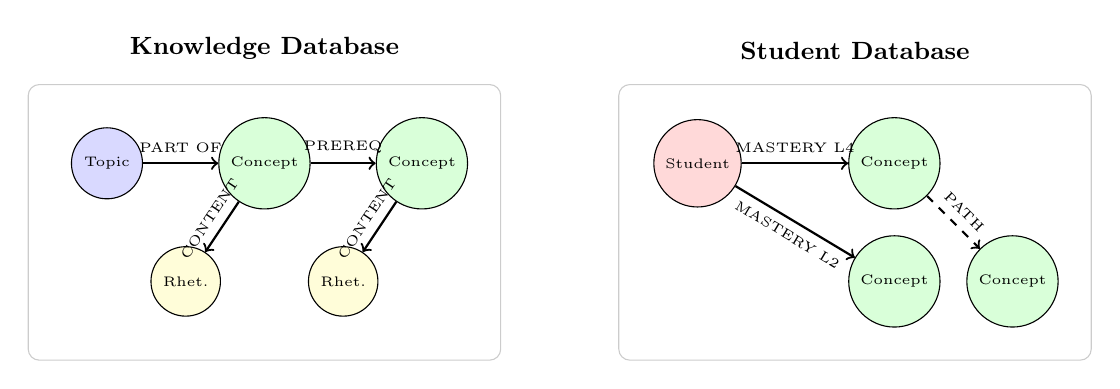
\begin{tikzpicture}[
  node distance=0.8cm,
  entity/.style={draw, circle, minimum size=0.8cm, font=\tiny, fill=#1},
  edge_lbl/.style={font=\tiny, midway, above, sloped},
  title/.style={font=\small\bfseries, anchor=south},
]
% Knowledge DB
\node[title] at (2.5, 3.2) {Knowledge Database};
\draw[gray!40, rounded corners] (-0.5,-0.5) rectangle (5.5,3.0);
\node[entity=blue!15] (c1) at (0.5, 2) {Topic};
\node[entity=green!15] (c2) at (2.5, 2) {Concept};
\node[entity=green!15] (c3) at (4.5, 2) {Concept};
\node[entity=yellow!15] (r1) at (1.5, 0.5) {Rhet.};
\node[entity=yellow!15] (r2) at (3.5, 0.5) {Rhet.};
\draw[->, thick] (c1) -- node[edge_lbl]{PART OF} (c2);
\draw[->, thick] (c2) -- node[edge_lbl]{PREREQ} (c3);
\draw[->, thick] (c2) -- node[edge_lbl]{CONTENT} (r1);
\draw[->, thick] (c3) -- node[edge_lbl]{CONTENT} (r2);
% Student DB
\node[title] at (10, 3.2) {Student Database};
\draw[gray!40, rounded corners] (7.0,-0.5) rectangle (13.0,3.0);
\node[entity=red!15] (s1) at (8.0, 2) {Student};
\node[entity=green!15] (sc1) at (10.5, 2) {Concept};
\node[entity=green!15] (sc2) at (12.0, 0.5) {Concept};
\node[entity=green!15] (sc3) at (10.5, 0.5) {Concept};
\draw[->, thick] (s1) -- node[edge_lbl]{MASTERY L4} (sc1);
\draw[->, thick] (s1) -- node[edge_lbl, below]{MASTERY L2} (sc3);
\draw[->, thick, dashed] (sc1) -- node[edge_lbl]{PATH} (sc2);
\end{tikzpicture}
    \vspace{12pt}\caption{Neo4j dual-database schema. Knowledge and learning graphs separated.}\label{fig:neo4j_schema}
\end{figure}

\subsubsection{Milvus: Vector Embedding Index}

The Milvus vector database stores 768-dimensional SciBERT embeddings generated during the knowledge ingestion pipeline. Each record in the collection consists of three fields described in Table~\ref{tab:milvus_schema}.

\begin{table}[H]
\centering
\caption{Milvus collection schema.}
\label{tab:milvus_schema}
\renewcommand{\arraystretch}{1.2}
\begin{tabularx}{\textwidth}{|l|l|l|X|}
\hline
\text{Field} & \text{Data Type} & \text{Constraint} & \text{Description} \\ \hline
id & VARCHAR & Primary Key & Unique entity identifier, shared with Neo4j for cross-database reference \\ \hline
text & VARCHAR & --- & Concatenation of concept name and content, used as the embedding source text \\ \hline
embedding & FLOAT\_VECTOR (768) & Indexed & SciBERT-generated dense vector for semantic similarity search \\ \hline
\end{tabularx}
\end{table}

The collection employs a Hierarchical Navigable Small World (HNSW) index optimised for the L2 (Euclidean) distance metric. Table~\ref{tab:hnsw_config} details the index and search parameters.

\begin{table}[H]
\centering
\caption{HNSW index configuration.}
\label{tab:hnsw_config}
\renewcommand{\arraystretch}{1.2}
\begin{tabularx}{\textwidth}{|l|l|X|}
\hline
\text{Parameter} & \text{Value} & \text{Purpose} \\ \hline
M (bi-directional links) & 8 & Maximum number of neighbours per graph node during index construction \\ \hline
efConstruction & 64 & Search depth during index build; higher values improve recall at the cost of build time \\ \hline
ef (query-time) & 64 & Search depth during query; balances retrieval accuracy against latency \\ \hline
Metric Type & L2 (Euclidean) & Distance metric for approximate nearest-neighbour search \\ \hline
\end{tabularx}
\end{table}

\subsubsection{MongoDB: Student State and Session Context}

MongoDB serves as the primary persistence layer for all student-related runtime data. Each student is represented as a single document keyed by their unique identifier, containing three major nested structures:

Table~\ref{tab:mongo_fields} provides the detailed field-level schema of the student document.

\begin{table}[H]
\centering
\caption{MongoDB student document field schema.}
\label{tab:mongo_fields}
\renewcommand{\arraystretch}{1.2}
\begin{tabularx}{\textwidth}{|l|l|X|}
\hline
Field Path & Type & Description \\ \hline
\multicolumn{3}{|l|}{\textit{state (Learning State)}} \\ \hline
finished\_communities & Array & List of completed knowledge graph communities \\ \hline
current\_pos & Object / null & Currently active concept node in the learning path \\ \hline
active\_resource & String / null & Currently loaded material reference \\ \hline
mastery\_map & Object & Key-value map of concept name to Bloom's mastery level (0--6) \\ \hline
previous\_nodes & Array & Ordered history of recently visited concept nodes \\ \hline
upcoming\_nodes & Array & Queue of next recommended concepts from roadmap \\ \hline
summary & String & Compressed natural-language summary of learning progress \\ \hline
pending\_proposal & Object / null & Unconfirmed learning path update awaiting student approval \\ \hline
\multicolumn{3}{|l|}{\textit{memo (Chat History) --- nested by session\_id}} \\ \hline
role & String & Speaker identifier: ``student'' or ``TA'' \\ \hline
heading & String & Topic heading for memo display \\ \hline
message & String & Full message content \\ \hline
timestamp & DateTime & Server-side UTC timestamp \\ \hline
\multicolumn{3}{|l|}{\textit{session\_context --- nested by session\_id and chat\_id}} \\ \hline
tool\_results & Array & Cached tool execution outputs for within-request recall \\ \hline
thoughts & Array & Agent reasoning traces for debugging and observability \\ \hline
\end{tabularx}
\end{table}

All write operations use atomic field-level updates (MongoDB \$set and \$push operators) rather than full document replacement. This ensures that concurrent sessions belonging to the same student can safely update disjoint fields (e.g., one session updating the mastery map while another appends to the chat memo) without overwriting each other's changes.

MinIO provides S3-compatible object storage for all binary educational assets. All objects reside in a single bucket named ``courses''. The storage hierarchy follows a deterministic three-level path convention detailed in Table~\ref{tab:minio_tree}, enabling the teaching workflow to reconstruct any object path programmatically from the concept's source reference property.

\begin{table}[H]
\centering
\caption{MinIO bucket directory structure.}
\label{tab:minio_tree}
\renewcommand{\arraystretch}{1.2}
\begin{tabularx}{\textwidth}{|l|l|X|}
\hline
\text{Path} &\text{ Content Type} & \text{Description} \\ \hline
\texttt{courses/} & Bucket root & Single top-level bucket containing all course data \\ \hline
\texttt{\{course\}/\{material\}/\{material\}.pdf} & application/pdf & Original raw PDF archived at ingestion time \\ \hline
\texttt{\{course\}/\{material\}/chunks/\{chunk\_id\}.txt} & text/plain & Extracted text chunk stored individually for granular retrieval \\ \hline
\end{tabularx}
\end{table}

The deterministic naming convention ensures that any component in the system can reconstruct an object path from two known values: the course name and the material name. The TA workflow exploits this property to serve PDF page references directly to the student frontend without querying a separate metadata index.

\subsubsection{SQLite: Authentication Store}

Student authentication is managed through a lightweight embedded SQLite database. Table~\ref{tab:sqlite_schema} describes the schema of the single ``students'' table.

\begin{table}[H]
\centering
\caption{SQLite students table schema.}
\label{tab:sqlite_schema}
\renewcommand{\arraystretch}{1.2}
\begin{tabularx}{\textwidth}{|l|l|l|X|}
\hline
\textbf{Column} &\textbf{Type}  & \textbf{Constraint} & \textbf{Description} \\ \hline
id & TEXT & PRIMARY KEY & Unique student identifier \\ \hline
username & TEXT & UNIQUE & Login credential, enforced unique \\ \hline
name & TEXT & --- & Student display name \\ \hline
email & TEXT & --- & Contact email address \\ \hline
password & TEXT & --- & SHA-256 hashed password \\ \hline
created\_at & TIMESTAMP & DEFAULT NOW & Account creation timestamp \\ \hline
\end{tabularx}
\end{table}

The deliberate choice of an embedded database eliminates external service dependencies for authentication while providing ACID guarantees for credential operations. Password hashing uses SHA-256 at the application layer before storage.

\subsection{Cross-Database Reference and Consistency}
Multiple system modules access to multiple database, and a lot of data of different source are aggregated and updated during run time.
To stabilize this structure, two architectural paradigms govern how the five storage engines coexist without data duplication or race conditions.

\subsubsection*{Unique Key Cross-Database Reference}

Entity identifiers serve as the primary cross-reference between Neo4j and Milvus: the same string identifier stored as a node 
property in Neo4j functions as the primary key in the Milvus collection, enabling the RAG agent to seamlessly translate between 
graph traversal results and vector similarity searches. When an agent performs a semantic search in Milvus, the returned identifiers are directly usable as lookup keys in Neo4j Cypher queries, eliminating the need for an intermediate translation layer.

Student identifiers bridge SQLite (authentication), MongoDB (learning state), and the Neo4j Student Database (mastery graph). 
A single login event propagates the authenticated identity consistently across all three stores: SQLite validates the credential 
and returns the student identifier, which MongoDB uses as its document primary key, and which Neo4j uses as the Student node 
property. This shared key ensures that mastery updates written by the TA workflow in Neo4j are immediately visible when the 
Student Tracker reads the learning state from MongoDB, without any synchronisation protocol beyond the identifier itself.

\subsubsection*{One-Write Policy}

With consistent cross-database reference, modules can easily access many database, a dangerous convenience that may hinge race condion risk. 
To solve this, "One-Write Policy" is proposed: 
each database collection or table is assigned exactly one write-owning module, with strictly governed method. All other modules 
are restricted to read-only access. Table~\ref{tab:write_policy} enumerates the write ownership assignments.

\begin{table}[H]
\centering
\caption{Write ownership per database.}
\label{tab:write_policy}
\renewcommand{\arraystretch}{1.2}
\begin{tabularx}{\textwidth}{|l|l|l|X|}
\hline
\textbf{Database} & \textbf{Collection} & \textbf{Writer} & \textbf{Consumers} \\ \hline
Neo4j (Knowledge) & Entity nodes, edges & Knowledge Module & TA Module \\ \hline
Neo4j (Student) & Student, MASTERY edges & TA Module & Student Module \\ \hline
Milvus & Concept embeddings & Knowledge Module & TA Module \\ \hline
MongoDB & students collection & Student Module & TA Module \\ \hline
MongoDB & learning\_logs collection & Student Module & TA Module \\ \hline
MinIO & courses bucket & Knowledge Module & TA Module \\ \hline
SQLite & students table & Student Module & --- \\ \hline
\end{tabularx}
\end{table}

This strict ownership eliminates the possibility of two modules concurrently writing to the same field. Combined with MongoDB's 
atomic field-level update operators, the policy ensures that even within a single write-owning module, concurrent sessions 
update disjoint document paths without overwriting each other's changes.


% ─────────────────────────────────────────────────────────────────────────────
\section{Student Module}
% ─────────────────────────────────────────────────────────────────────────────

\subsection{Authentication: OAuth2 + JWT}

The student module implements a standard OAuth2 password flow using  {PyJWT} for JWT minting. The  {/student/login} endpoint 
validates credentials against SHA-256 hashed passwords in SQLite and returns a short-lived JWT ( {sub} =  {student\_id}). All 
subsequent requests attach this token as a Bearer credential;  {get\_current\_student()} (a FastAPI dependency) decodes and 
validates it on each call.

\subsection{Session Lifecycle and the Identity Firewall}\label{sec:firewall}

The idea of this module is to initiate access to sensitive components and resources and enable logic modules only after login, via a controlled restricted manner. 
Moreover, it must guarantee an abstracted, hidden access that cannot be fully comprehend from application layer, but can only invoke via monitored request protocols.

The discussed paradigms goes into practice by a authentication and permission granted through a session lifecycle design described in Figure~\ref{fig:student_login}. The 
proccess goes by:
\begin{enumerate}
  \item After login, the student calls  {POST /student/session/start} with their JWT. The server generates a random UUID ( {session\_id}) and registers it in  {Student\_Tracker}.
  \item All subsequent TA interactions supply only  {session\_id}. The TA Module never receives  {student\_id}.
  \item Inside  {Student\_Tracker.\_resolve()}, the private mapping  {session\_id → student\_id} translates transparently before any database call.
\end{enumerate}


\begin{figure}[H]
\centering
\resizebox{\textwidth}{!}{%
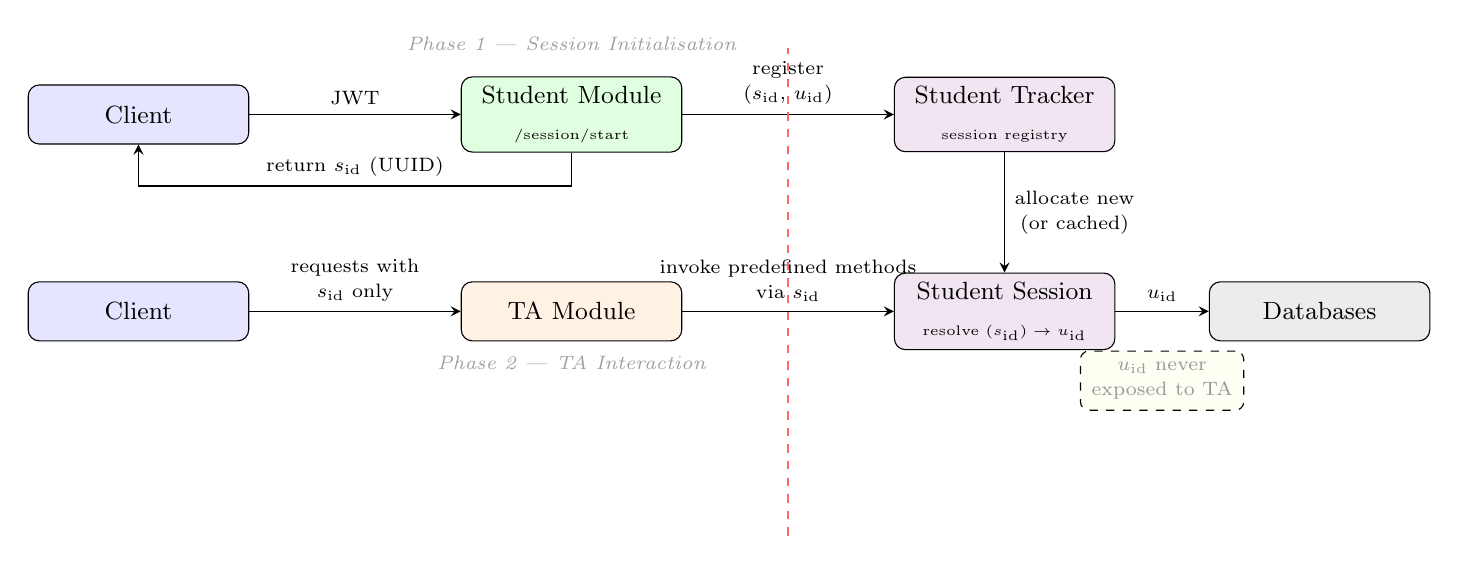
\begin{tikzpicture}[
  every node/.style={font=\small},
  box/.style={draw, rounded corners=4pt, minimum width=2.8cm, minimum height=0.75cm,
              align=center, fill=#1},
  arr/.style={->, >=stealth, semithick},
  lbl/.style={font=\scriptsize, align=center}, 
]
%% ── Phase 1: Session Initialisation ────────────────────────────────────
\node[box=blue!10]    (C1)  at (0,   2.5) {Client};
\node[box=green!12]   (SS)  at (5.5, 2.5) {Student Module\\[2pt]{\tiny /session/start}};
\node[box=violet!10]  (ST1) at (11.0, 2.5) {Student Tracker\\[2pt]{\tiny session registry}};

\draw[arr] (C1) -- node[above, lbl]{JWT} (SS);
\draw[arr] (SS) -- node[above, lbl]{register\\[1pt]$(s_\mathrm{id},\, u_\mathrm{id})$} (ST1);

\draw[arr] (SS.south) -- ++(0,-0.42) -- ++(-5.5, 0) -- (C1.south);
\node[lbl, below] at (2.75, 2.08) {return $s_\mathrm{id}$ (UUID)};

%% ── Phase 2: TA Interaction ─────────────────────────────────────────────
\node[box=blue!10]    (C2)  at (0,    0)  {Client};
\node[box=orange!10]  (TA)  at (5.5,  0)  {TA Module};
\node[box=violet!10]  (ST2) at (11.0,  0)  {Student Session\\[2pt]{\tiny resolve $(s_\mathrm{id}) \to u_\mathrm{id}$}};
\node[box=gray!15]    (DB)  at (15.0, 0)  {Databases};

\draw[arr] (C2)  -- node[above, lbl]{requests with\\[1pt]$s_\mathrm{id}$ only} (TA);
\draw[arr] (TA)  -- node[above, lbl]{invoke predefined methods\\[1pt]via $s_\mathrm{id}$} (ST2);
\draw[arr] (ST2) -- node[above, lbl]{$u_\mathrm{id}$} (DB);
\draw[arr] (ST1)  -- node[right, lbl]{allocate new\\[1pt](or cached)} (ST2);

%% ── Identity Firewall ───────────────────────────────────────────────────
\draw[dashed, thick, red!60] (8.25, -2.85) -- (8.25, 3.35);


%% ── Phase labels ────────────────────────────────────────────────────────
\node[font=\scriptsize\itshape, text=gray!75] at (5.5,  3.4)
    {Phase 1 --- Session Initialisation};
\node[font=\scriptsize\itshape, text=gray!75] at (5.5, -0.65)
    {Phase 2 --- TA Interaction};

%% ── Annotation ──────────────────────────────────────────────────────────
\node[draw, dashed, rounded corners=3pt, font=\scriptsize, text=gray!80,
      align=center, inner sep=4pt, fill=yellow!5] at (13.0, -0.88)
    {$u_\mathrm{id}$ never\\[1pt]exposed to TA};
\end{tikzpicture}%
}
    \vspace{12pt}\caption{Login protocol with Identity Firewall (represented by the red line).}\label{fig:student_login}
\end{figure}

This pattern is analogous to a hotel key-card system: the key (session\_id) grants access to resources, but revealing it does not expose the guest's credentials 
(student\_id). Most importantly, all modules, tools can only gain abstracted access to student metadata can only be done once login. This prevent dangerous activity 
from AI or outside parties to sensible databases and resources.

As such, {Student Tracker} acts as a Singleton Manager that provide, cache and clean resources of unused Session. In the current implementation, 
it manages two distinct layers of state:

\begin{enumerate}
    \item {Session-Specific State ( {StudentSession})}: Keyed by  {session\_id}, this layer isolates chat history and session-specific context (like recent PDF pages). This prevents "Identity Race Conditions" where multiple browser tabs contaminate each other's chat logs.
    \item {Shared Learning State}: Keyed by  {student\_id}, this layer caches the student's learning progress (current position, mastery map, etc.) and is shared across all active sessions of the same student.
\end{enumerate}

To ensure data integrity during concurrent updates, the tracker utilizes {Atomic Field Updates} in MongoDB. 
Instead of overwriting the entire state object, the system updates specific fields (e.g., updating only the  {current\_pos} or appending to  {finished\_communities}). 
This design effectively mitigates "Data Race Conditions" where one session might accidentally revert progress made in another concurrent session.

% ─────────────────────────────────────────────────────────────────────────────
\section{Knowledge Module}\label{sec:knowledge_module}
% ─────────────────────────────────────────────────────────────────────────────

The Knowledge Module operates as an offline administrative pipeline responsible for transforming raw educational documents into the structured Educational Knowledge Graph consumed by the Teaching Assistant at runtime. This module is accessible exclusively through a dedicated REST endpoint, invoked by administrators upon uploading new course materials.

\subsection{Technical Setup}

Table~\ref{tab:km_libs} summarises the principal libraries employed by the Knowledge Module. All dependencies are resolved through the \textit{uv} package manager, ensuring deterministic, lockfile-driven builds across development and deployment environments.

\begin{table}[H]
\centering
\caption{Knowledge Module core libraries.}
\label{tab:km_libs}
\renewcommand{\arraystretch}{1.3}
\begin{tabularx}{\textwidth}{|l|X|}
\hline
\textbf{Library} & \textbf{Role in Pipeline} \\ \hline
Docling & PDF parser that converts each page into structured text blocks with provenance metadata such as page number and bounding region. \\ \hline
spaCy & Natural language processing library providing lemmatisation, synonym resolution, and stopword filtering for the post-extraction deduplication stage. \\ \hline
Pydantic & Schema validation framework that enforces strict structural contracts on every LLM extraction output, rejecting malformed responses before graph insertion. \\ \hline
SciBERT & Domain-specific sentence transformer (768 dimensions) trained on scientific corpora, generating embeddings that capture academic semantic similarity. \\ \hline
\end{tabularx}
\end{table}

\subsection{Ingestion Workflow}

The ingestion pipeline supports two distinct material types---lecture slides and textbooks---each following a tailored processing path. Both paths share a common entry stage (document parsing and window segmentation as described in Section~\ref{subsub:sliding}), but diverge at the knowledge extraction stage due to the fundamentally different structural roles these materials serve in the educational knowledge base.

To maximize throughput and minimize hardware idle time, both pipelines are engineered as fully asynchronous systems. This architectural choice prevents blocking operations during heavy I/O tasks or Large Language Model (LLM) inference, effectively turning a sequential bottleneck into a continuous stream of data processing.

\begin{figure}[H]
\centering
\resizebox{0.95\textwidth}{!}{%
\begin{tikzpicture}[
    >=stealth, font=\sffamily,
    % Styles
    threadBox/.style={draw, thick, rounded corners=8pt, inner sep=15pt},
    actionNode/.style={draw, thick, fill=white, rounded corners=4pt, minimum width=2.8cm, minimum height=0.8cm, align=center},
    queueNode/.style={draw, thick, rounded corners=10pt, minimum width=3.5cm, minimum height=1cm, align=center},
    dbNode/.style={draw, thick, fill=gray!15, cylinder, shape border rotate=90, aspect=0.25, minimum width=1.4cm, minimum height=1.2cm, align=center}
]

% ================= DATABASES (Bờ ngoài cùng) =================
\node[dbNode] (minio) at (0, 4) {\textbf{MinIO}};
\node[dbNode] (neo) at (5, 0.0) {\textbf{Neo4j}};

% ================= CỘT 1: MAIN THREAD (Non-blocking) =================
\node[actionNode, draw=blue!80] (pdf) at (0, 6.5) {\textbf{pdf extractor}\\};
\node[actionNode, dashed, draw=gray, text=gray] (other) at (0, 1.5) {\textit{Main Thread Free}\\\textit{(Repeat PDF extraction...)}};

% ================= CỘT 2: MIDDLEWARE QUEUES (Buffer) =================
\node[queueNode, fill=purple!10, draw=purple!60] (q1) at (5, 6.5) {\texttt{extract\_queue}\\(Chunk Buffer)};
\node[queueNode, fill=green!10, draw=green!60] (q2) at (5, 4) {\texttt{build\_queue}\\(Graph Buffer)};

% ================= CỘT 3: ASYNC WORKER POOL =================
% 1. Parallel LLM Workers (Vẽ 3 hộp đè lên nhau tạo hiệu ứng Parallel)
\node[actionNode, fill=orange!10, draw=orange!80] (w3) at (10.6, 6.9) {\textbf{LLM Worker 2}};
\node[actionNode, fill=orange!10, draw=orange!80] (w2) at (10.8, 6.7) {\textbf{LLM Worker 1}};
\node[actionNode, fill=orange!10, draw=orange!80] (w1) at (11.0, 6.5) {\textbf{LLM Worker 0}};

% 2. Sequential Graph Constructor
\node[actionNode, fill=teal!10, draw=teal!80] (gc) at (5, 2.25) {\textbf{Graph Constructor}\\(Sequential)};


% ================= TIMELINE (Trục dọc) =================
\draw[->, thick, gray] (13, 7.5) -- (13, 0);
\node[right, font=\small] at (13, 6.5) {Time $t_0$};
\node[right, font=\small] at (13, 4.75) {Time $t_1$};
\node[right, font=\small] at (13, 3) {...............};
\node[right, font=\small] at (13, 1) {Time $t_n$};

% ================= ARROWS & ROUTING =================
% Main Thread activities
\draw[->, thick, blue!80] (pdf.south) -- (minio.north) node[midway, above, font=\scriptsize] {upload\_raw};
\draw[->, thick, blue!80] (pdf.east) -- (q1.west) node[midway, above, font=\scriptsize] {put(chunk)};
\draw[->, thick, dashed, gray] (minio.south) -- (other.north) node[midway, right, font=\scriptsize, align=left] {Keep running, No waiting};

% Queue 1 to Workers
\draw[->, thick, orange!80] (q1.east) -- (w1.west) node[midway, above, font=\scriptsize] {get()};

% Workers to Queue 2 (Đường chéo vắt ngược lại Buffer)
\draw[->, thick, orange!80] (w1.south) -- (q2.north east) node[midway, above right, font=\scriptsize, xshift=0.3cm] {put(sub-graph)};

% Queue 2 to Graph Constructor
\draw[->, thick, teal!80] (q2.south) -- (gc.north) node[midway, above, font=\scriptsize] {get()};

% Graph Constructor to Neo4j
\draw[->, thick, teal!80] (gc.south) -- (neo.north) node[midway, above, font=\scriptsize] {update()};

\end{tikzpicture}%
}
\vspace{15pt}\caption{Asynchronous Ingestion Pipeline integrating Queues, Parallel Workers, and Storage}
\label{fig:ingestion}
\end{figure}

Lecture slides follow the primary extraction path. Because slide extraction involves complex, interdependent LLM operations and strict database insertion rules, it is architected as a Three-Station Producer-Consumer pipeline interconnected by bounded asynchronous queues. This design guarantees that data extraction happens continuously without being bottlenecked by slower downstream database operations.

\begin{itemize}
    \item \textbf{Station 1 (Producer):} The operation on the main threads continuously parses the PDF document, chunking pages and immediately uploading the raw segments 
    to MinIO. As soon as a chunk is ready, it is pushed into the Extraction Queue, then it leaves all the work to the background consumer and move the next document.
    \item \textbf{Station 2 (LLM Workers):} A pool of concurrent worker coroutines consumes items from the Extraction Queue. These workers operate independently, 
    forwarding chunks to the LLM for the Dual-Phase Extraction (concept mapping and relation discovery). The asynchorous task are yielded to wait for the LLM 
    result from cloud, costing little memory but effectively reduces inference waiting times. Once the LLM yields the structural representation, the result is 
    forwarded to the Build Queue.
    \item \textbf{Station 3 (Graph Builder):} A single sequential getting extracted nodes, edges result from the Build Queue. It constructs the Knowledge Graph 
    and ensures safe, transaction-free graph updates to Neo4j. Keeping this station single-threaded intentionally prevents race conditions and topological conflicts 
    during the graph assembly phase, while the heavier workload (LLM inference) remains aggressively parallelized upstream.
\end{itemize}

Backpressure mechanisms are naturally enforced by setting maximum capacity limits on the interconnecting queues, ensuring that memory usage remains stable even if the 
PDF parsing station outpaces the LLM workers. Experiments shows that results are 30\% faster with this approach.


\subsection{Graph Schema at Database Level}

The Knowledge Graph stored in Neo4j follows the formal Property Graph definition established in Section~\ref{sub:g_def}. Each entity node carries a set of standardised properties that support both structural navigation and semantic retrieval:

\begin{table}[H]
\centering

\renewcommand{\arraystretch}{1.2}
\begin{tabularx}{\textwidth}{|l|X|}
\hline
Property & Description \\ \hline
Name & Canonical concept label, enforced unique across the database \\ \hline
Identifier & Machine-generated unique key for programmatic reference \\ \hline
Content & Full textual description or definition of the concept \\ \hline
Node Type & Ontological category: Community, Topic, Concept, or Rhetorical \\ \hline
Rhetorical Role & Instructional function (Definition, Theorem, Application), assigned only to Rhetorical-type nodes \\ \hline
Cluster & Community identifier assigned during graph construction \\ \hline
Source Reference & Serialised pointer to the original material location in object storage \\ \hline
\end{tabularx}
\vspace{12pt}\caption{Entity node properties in Neo4j.}
\label{tab:node_props}
\end{table}

Five directed edge types connect these entities: \textit{PART OF} (hierarchical containment), \textit{RELATED TO} (semantic association), \textit{PREREQUISITE OF} (learning dependency), \textit{CONTENT} (rhetorical elaboration from concept to its explanatory nodes), and \textit{ELABORATES ON} (textbook enrichment). The database enforces structural integrity through four constraints: unique identifiers, unique names, a full-text search index across both fields, and a dedicated index on the rhetorical role property for role-filtered retrieval queries.

% ─────────────────────────────────────────────────────────────────────────────
\section{Teaching Assistant Module}\label{sec:ta_module}
% ─────────────────────────────────────────────────────────────────────────────

The Teaching Assistant (TA) Module is the real-time component of the system, responsible for processing student queries and generating pedagogically grounded responses by orchestrating tool-calling agents across a state-driven workflow. Unlike the Knowledge Module which operates offline, the TA Module handles concurrent student sessions with sub-second latency requirements.

\subsection{Technical Setup}

\begin{table}[H]
\centering
\caption{TA Module core libraries.}
\label{tab:ta_libs}
\renewcommand{\arraystretch}{1.3}
\begin{tabularx}{\textwidth}{|l|X|}
\hline
Library & Role in Module \\ \hline
LangGraph & Workflow graph builder providing typed state containers, conditional routing, and compiled sub-graph composition for deterministic agent orchestration. \\ \hline
LangChain & Agent abstraction layer supplying tool binding, middleware protocol, structured output parsing, and the ReAct execution loop. \\ \hline
Pydantic & Structured output schemas ensuring every agent response conforms to a predefined contract before reaching the student. \\ \hline
asyncio & Non-blocking concurrent execution enabling background persistence, parallel database writes, and real-time streaming without blocking the response pipeline. \\ \hline
\end{tabularx}
\end{table}

In a conventional single-agent architecture of many framework including, the system prompt, context, and tools are fixed at initialization---forcing the model to simultaneously 
manage routing, retrieval, evaluation, and generation instructions, which degrades performance as task complexity grows. 
\begin{figure}[H]
    \centering
    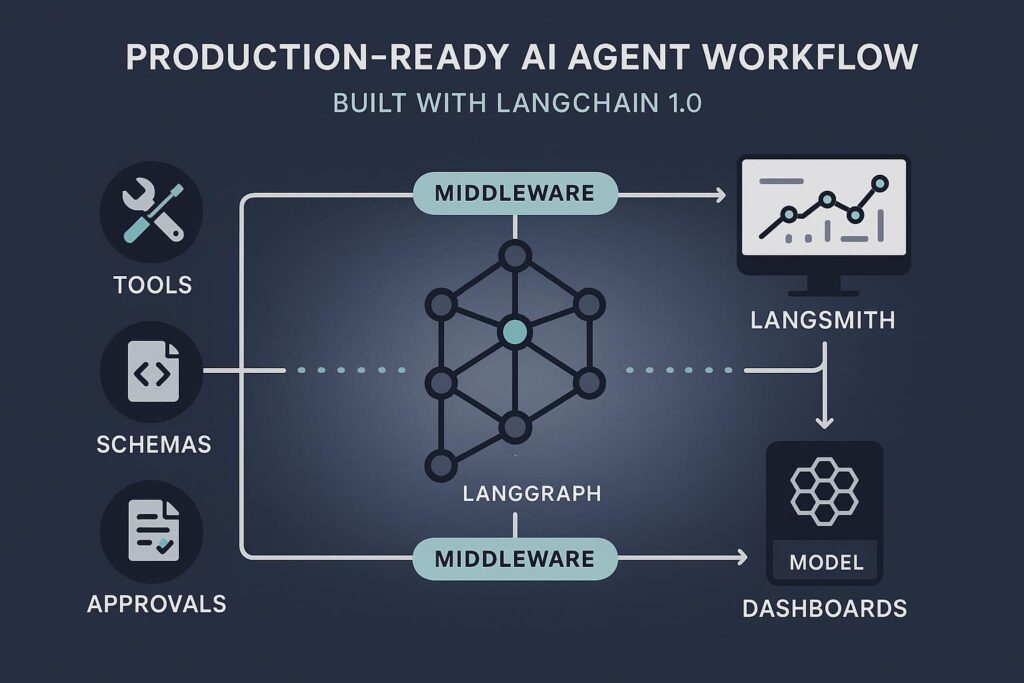
\includegraphics[width=0.5\textwidth]{Images/system/lang_mid.jpg}
    \vspace{12pt}\caption{Practice of Langchain Middleware Integration, inspired by \href{https://skywork.ai/blog/ai-agent/best-practices-langchain-1-0-production-ready-llm-apps/}{How LangChain 1.0 Simplifies Building Production-Ready LLM Applications}}}\label{fig:lang_mid}
\end{figure}
Langchain Middleware~\cite{LangMid}, released in December 2025, is one of the latest features providing a composable interceptor that modifies the model's request before it reaches the language model, 
enabling a single agent to exhibit distinct behaviours per workflow node. Unlike role-based frameworks where changing an agent's behaviour requires spawning 
a new instance entirely, the middleware approach eliminates redundant model connections while preserving per-node specialisation. The Figure~\ref{fig:lang_mid} 
demonstrates the reference to the practice of LangChain Middleware Integration.

\subsection{LangGraph Workflow Design}

The TA Module's orchestration layer is built as a LangGraph state machine where each node represents either a specialised processing step or a compiled sub-workflow. 
For each node design, the components within the schema orchestrate data flow through two primary mechanisms. As the agent state and student state traverse 
the nodes alongside runtime configurations, an exclusion mechanism is applied: the system filters the context so that each agent only sees the information strictly necessary for its current task, keeping the prompt clean and preventing interference from irrelevant data.
\begin{figure}[H]
    \centering
    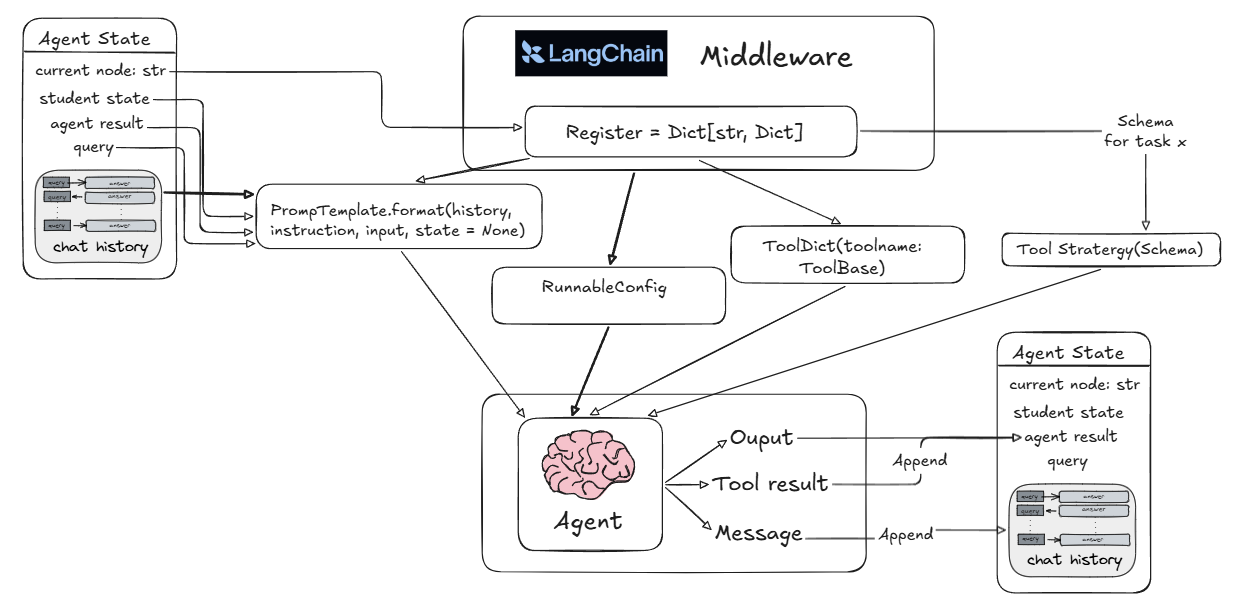
\includegraphics[width=\textwidth]{Images/system/langchain_node.png}
    \vspace{12pt}\caption{Standard operation of a LangGraph Node}\label{fig:lang_node}
\end{figure}
\paragraph*{AgentState:} Representing the dynamic data payload and memory of the system.
\begin{itemize}
  \item Query: Input from the user
  \item Agent result: Other Agents non message results accumulated from previous nodes in the workflow such as intermediate reasoning, tool results buffer.
  \item Chat history: An array containing the conversation history results.
  \item Current Node: name of the current node, used to find its pre\-registered means and resources in the Register
\end{itemize}

\paragraph*{Middleware:} Building upon the core middleware framework, the system applies the Adaptive Middleware pattern inherited from Langchain. My design ties its
behaviour with the Register, which is a nested dictionary. The LangGraph Node name act as a key to access an inner dictionary containing the following items:
\begin{itemize}
  \item Prompt Template: Created by LangChain PromptTemplate. Constructs AgentState and Query by combining predefined Meta Context and task instruction, 
  forming a detailed instruction set to invoke agents. For TA, the Prompt template include chat history and optionally agent result
  \item Tools: Grouped according to task and registered during initialization.
  \item ToolStrategy: Override schema runtime during
  \item Runnable Config: Registered configurations that change agent behaviour according to the task. For example, enforcing low temperatures for rigid retrieval tasks.
\end{itemize}
The Middleware use the node name to get the dictionary, then pass it to the built\-in Langchain call() method overriding agent calls, redefining agent behaviour and output.
Agent output will append to Agent State as in the figure. This ensure state and context management across the whole workflow, while still preserve local context and agentic
behaviour in that local setting.


% ─────────────────────────────────────────────────────────────────────────────

% ─────────────────────────────────────────────────────────────────────────────
\subsection{Tracing and Observability}\label{sub:tracing}
% ─────────────────────────────────────────────────────────────────────────────

Agentic systems is an unstable and blackbox pipeline. Ensuring system in production requires comprehensive observability of agentic input, output and all intermediate step including reasoning chain 
to diagnose reasoning failures, measure latency bottlenecks, and audit the decision-making process. The Tracing Module captures a structured record of every agent 
interaction, providing both local persistence for debugging and long-term monitoring.

The tracing system organises observability data into a three-level hierarchy, illustrated in Figure~\ref{fig:trace_model}. Each level captures progressively finer-grained information about the agent's execution.

\begin{figure}[H]
\centering
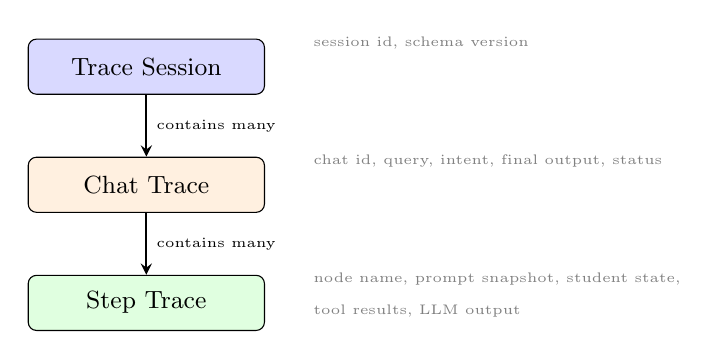
\begin{tikzpicture}[
  level/.style={draw, rounded corners=3pt, minimum width=3.0cm, minimum height=0.7cm, align=center, font=\small, fill=#1},
  arr/.style={->, >=stealth, thick},
  contains/.style={font=\tiny, midway, right},
]
\node[level=blue!15] (session) at (0, 2) {Trace Session};
\node[level=orange!12] (chat) at (0, 0.5) {Chat Trace};
\node[level=green!12] (step) at (0, -1) {Step Trace};
\draw[arr] (session) -- node[contains]{contains many} (chat);
\draw[arr] (chat) -- node[contains]{contains many} (step);
% Fields
\node[font=\tiny, anchor=west, text=gray] at (2.0, 2.3) {session id, schema version};
\node[font=\tiny, anchor=west, text=gray] at (2.0, 0.8) {chat id, query, intent, final output, status};
\node[font=\tiny, anchor=west, text=gray] at (2.0, -0.7) {node name, prompt snapshot, student state,};
\node[font=\tiny, anchor=west, text=gray] at (2.0, -1.1) {tool results, LLM output};
\end{tikzpicture}
    \vspace{12pt}\caption{Trace data hierarchy. Three nested observation levels.}\label{fig:trace_model}
\end{figure}

At the top level, a Trace Session spans the student's entire connected session and serves as the root container. Each student message creates a Chat Trace 
containing the original query, the classified intent, and the final response. Within each chat, Step Traces record the execution of each workflow node: 
the prompt to invoke language model (truncated for context window fit and storage effieciency), a snapshot of the AgentState at that moment containing 
student's learning state , any tool execution results, and the model's output.

Each active session maintains an in-memory trace buffer. As workflow nodes execute, each node appends a step record to the current chat's buffer. When a chat turn 
completes, the full session trace is serialised to JSON and written to a persistent file. The writer employs dual locking mechanisms---a threading lock for synchronous 
contexts and an asynchronous lock for coroutine contexts---ensuring thread safety when multiple workflow nodes attempt concurrent trace writes.

For production monitoring, the system integrates with Langfuse, a cloud-based observability platform built for LLM applications. 
The integration operates through LangChain's callback protocol: a Langfuse callback handler is injected into the runtime configuration at a 
session starts, automatically capturing every LLM invocation, tool call precisely from inner system.